\documentclass[11pt]{article}
\usepackage[margin=1in]{geometry}
\usepackage[T1]{fontenc}
\usepackage[utf8]{inputenc}
\usepackage{lmodern}
\usepackage{microtype}
\usepackage{graphicx}
\usepackage{amsmath,amssymb}
\usepackage[numbers,sort&compress]{natbib}
\usepackage{booktabs}
\usepackage{enumitem}
\usepackage{hyperref}
\hypersetup{colorlinks=true,linkcolor=blue,citecolor=blue,urlcolor=blue}
\setlength{\parskip}{5pt}
\setlength{\parindent}{0pt}
\title{Enhancing PCAP-Backdoor: A Methodology for Multi-Signal Detection, Robust Retraining, Generalization, and Runtime Evaluation}
\author{R. U. Vijay Pranav\\CS23B1073\\B1 -- Btech\\Department of Computer Science and Engineering, Indian Institute of Information Technology Design and Manufacturing Kancheepuram, India}
\date{Research Methodology Paper\\November 2026}
\begin{document}
\maketitle
\begin{abstract}
Deep learning-based intrusion detection systems (IDS) for cyber-physical systems (CPS) and the Internet of Things (IoT) can be vulnerable to training-time backdoor poisoning. PCAP-Backdoor, introduced by Chathoth et al. \cite{ref1}, demonstrates a packet-level attack in which protocol-conforming trigger packets are inserted into raw packet-capture (PCAP) traffic before feature extraction. The attack is significant because it targets the packet-to-feature pipeline rather than requiring direct modification of the feature vectors. This paper proposes a methodology for extending the defensive and evaluative components of PCAP-Backdoor while retaining its original threat model and attack pipeline as the reference framework. Four extensions are specified: (i) a multi-signal detection design combining activation- space analysis, device-relative feature consistency, prediction-confidence measures, and temporal traffic indicators; (ii) a robust retraining strategy combining class-aware sampling, gradual introduction of correctly labelled trigger- bearing examples, and clean-sample replay; (iii) a generalization protocol using random, device-disjoint, and chronological splits with repeated runs and leakage controls; and (iv) a deployment-oriented profiling protocol for latency, throughput, processor use, and memory consumption. The paper defines the proposed components, their interfaces, evaluation metrics, baselines, ablations, and validity considerations. No new implementation or experimental evaluation is claimed. All proposed improvements remain hypotheses to be tested, and no performance advantage over the original PCAP-Backdoor framework is asserted.
\end{abstract}
\noindent\textbf{Keywords---}backdoor attacks, network intrusion detection, PCAP, clean-label poisoning, CPS security, IoT security, activation clustering, adversarial retraining, generalization, runtime profiling.

\section{Introduction}
The convergence of information technology and operational technology has increased the connectivity of cyber- physical systems (CPS), industrial control systems, and Internet of Things (IoT) deployments. These environments depend on network communication for monitoring, control, and service delivery, making traffic analysis an important component of their security architecture. Machine-learning-based intrusion detection systems can learn patterns from network observations, but their practical reliability depends on the quality, representativeness, and integrity of the training data \cite{ref2}. Backdoor poisoning is a training-time threat in which an adversary causes a model to associate a particular trigger with an attacker-selected prediction. The resulting model may retain apparently normal performance on ordinary inputs while behaving incorrectly when the trigger is present. BadNets established a widely studied example of this class of vulnerability \cite{ref3}. Subsequent work has developed detection and mitigation methods, including activation clustering, spectral analysis, trigger reconstruction, and pruning-based approaches \cite{ref4}--\cite{ref7}.

Network IDS introduce a distinctive attack surface because many classifiers do not consume raw packets directly. Instead, packet captures are transformed into flow- or channel-level feature vectors. Kitsune, for example, combines an online feature-extraction framework with an ensemble of autoencoders for anomaly detection \cite{ref8}. The PCAP- Backdoor framework addresses this packet-to-feature boundary: Chathoth et al. \cite{ref1} describe how protocol- conforming packets can be inserted into raw traffic so that downstream feature statistics are altered without direct access to the feature extractor. The present work does not propose a new packet trigger or replace the original attack. It focuses on four aspects of the surrounding defensive and evaluation methodology that warrant further study: detection beyond a single activation-space test; retraining strategies that explicitly preserve clean-task performance; evaluation under data partitions that better reflect device and time separation; and measurement of operational cost. These extensions are motivated by the original framework and by established concerns about the validity and deployability of machine- learning-based network intrusion detection \cite{ref2}. The contribution is a structured research proposal. It defines (1) a multi-signal detector with separate training-data sanitization and inference-time operating modes; (2) a three-part robust retraining procedure; (3) a leakage-aware, multi-seed evaluation design; and (4) a stage-wise runtime profiling protocol. The proposed methods are not presented as validated defenses. Their effectiveness, overhead, and limitations require implementation and empirical evaluation.

\section{Related Work}
\subsection{Backdoor attacks in deep learning}
Gu et al. \cite{ref3} demonstrated that a model can maintain ordinary classification behavior while responding to attacker- selected trigger patterns with an unintended output. This established the model-supply-chain and training-data integrity implications of backdoor learning. Backdoor research has since examined trigger construction, poisoning constraints, transferability, and model inspection. These studies provide the conceptual foundation for considering the integrity of training data as part of IDS security.

\subsection{Backdoors in network-traffic classifiers}
Network-traffic classifiers differ from image and text models because their inputs are often derived from packets through protocol parsing, flow construction, and statistical feature extraction. TrojanFlow studies a neural backdoor attack against deep-learning network-traffic classifiers \cite{ref9}. PCAP-Backdoor \cite{ref1} focuses specifically on manipulating raw packet captures before feature extraction, thereby addressing a different point in the processing chain. The distinction matters: defenses that assume direct access to a feature vector may not be directly applicable when an attacker can only contribute packet-level traffic.

\subsection{Backdoor detection and mitigation}
Activation clustering examines hidden-layer representations to identify potentially distinct poisoned and clean subpopulations \cite{ref4}. Neural Cleanse attempts to reconstruct unusually small triggers associated with target classes \cite{ref5}, while spectral-signature methods search for statistical outliers in learned representations \cite{ref6}. Fine-pruning combines neuron pruning with subsequent fine-tuning as a backdoor mitigation strategy \cite{ref7}. These approaches were not all designed for packet-derived IDS features. Their assumptions, detection granularity, and operational cost therefore need to be evaluated in the target traffic domain rather than transferred without validation.

\subsection{Feature extraction and network IDS evaluation}
Kitsune provides an online network feature-extraction and anomaly-detection framework and is relevant to the feature-processing context used by PCAP-Backdoor \cite{ref8}. The associated Kitsune Network Attack dataset contains multiple network-attack captures and provides packet-level feature records alongside truncated PCAP captures \cite{ref10}. The dataset documentation states that its PCAP files are truncated to 200 bytes for privacy. Consequently, any packet-level reconstruction or payload-sensitive analysis using those captures must account for the truncation and verify which packet fields remain usable.

Sommer and Paxson emphasize that network intrusion detection presents evaluation challenges that differ from many conventional machine-learning tasks, including changing traffic distributions, operational costs, and difficulty obtaining representative data \cite{ref2}. Random splitting can be useful for reproducing an existing benchmark, but it does not alone establish performance on unseen devices or later traffic. This motivates reporting multiple split regimes and treating the split strategy as part of the experimental question.

\subsection{Positioning of the proposed work}
This paper is an extension proposal for the defensive and evaluation methodology surrounding PCAP-Backdoor. It does not claim that the individual techniques---activation clustering, confidence scoring, robust sampling, or chronological testing---are new in isolation. The proposed contribution is their structured integration around a raw- PCAP backdoor threat model, together with explicit separation of pre-training sanitization, inference-time monitoring, robust retraining, generalization testing, and resource profiling.

\section{Original PCAP-Backdoor Framework}
\subsection{Threat model}
PCAP-Backdoor considers a victim who trains a deep-learning IDS using network traffic and an attacker who can contribute or manipulate a subset of training traffic. The central restriction is that the attacker operates at the raw- packet level and does not directly edit the feature vectors produced by the victim's extractor. The attack is described as clean-label: the contributed traffic retains its benign label, while the intended effect is to cause trigger-bearing malicious traffic to be classified as a target class. The framework also considers a black-box setting in which the attacker lacks detailed knowledge of the victim's model architecture and training procedure \cite{ref1}.

\subsection{Packet-level trigger generation}
The original framework inserts trigger packets into benign packet streams according to parameters described in the source paper, including trigger count (B), inter-packet delay (D), injection ratio or probability (R), and packet payload-length handling (L). The generator distinguishes traffic contexts and constructs packets intended to remain sufficiently protocol-conforming for subsequent packet processing. The important methodological point is that the manipulation occurs before feature extraction: the attacker attempts to influence downstream packet-size, timing, and channel statistics indirectly \cite{ref1}. This paper retains that attack-generation procedure as the reference and does not introduce a new trigger algorithm.

\subsection{Feature extraction and classification}
The original study uses packet-derived statistical features, including the Kitsune feature-extraction approach, and evaluates deep neural classifiers. The supplied draft identifies DNN-3 as the primary model and describes a 115- input architecture with hidden-layer widths of 128, 64, 32, and 16 before the output layer. Because architectural descriptions and experimental configurations must be checked against the final published article before submission, these details should be treated as the configuration reported in the working source draft and verified against \cite{ref1}.

\subsection{Datasets and reported findings}
\begin{figure}[htbp]\centering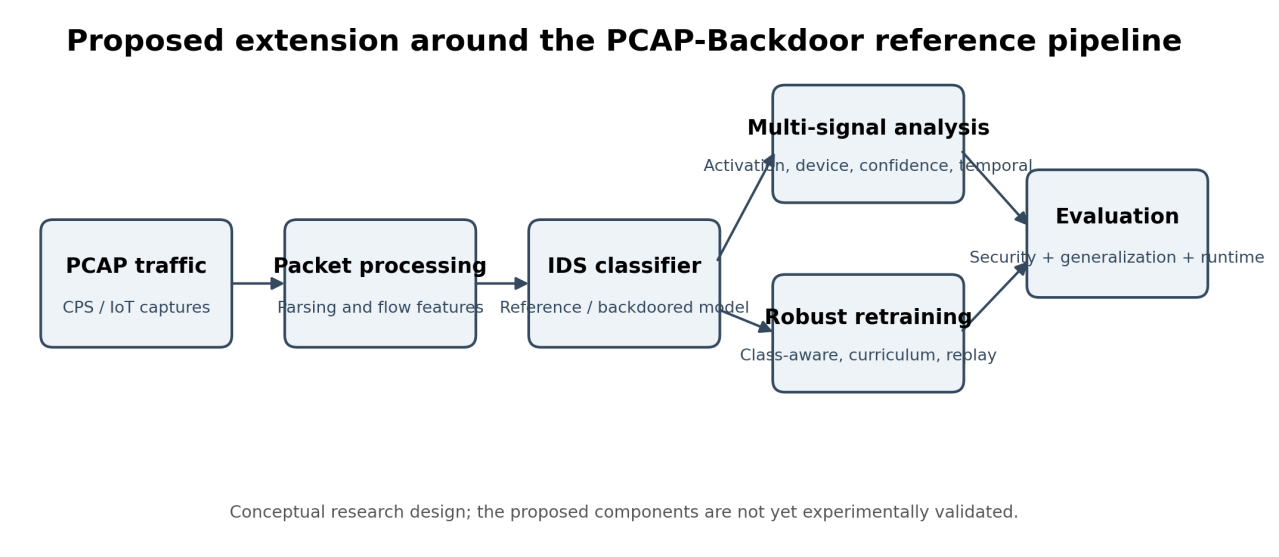
\includegraphics[width=0.92\linewidth]{images/figure1.png}\caption{Proposed research extension surrounding the original PCAP-Backdoor pipeline. The diagram is conceptual and does not report experimental outcomes.}\end{figure}
The original paper reports evaluation on CPS/SCADA traffic and IoT network traffic. It reports that a small poisoned fraction can induce high attack success in several settings and evaluates activation clustering, adversarial retraining, and neural pruning as defenses \cite{ref1}. The exact values, class definitions, split construction, and per-dataset configurations should be cited directly to the relevant tables and figures of the original publication in any camera- ready version. This paper does not reproduce those measurements and does not treat them as results of the proposed extensions. A dataset distinction is important for future evaluation. The UCI Kitsune Network Attack resource describes nine captures spanning attacks such as fuzzing, ARP MitM, active wiretap, and Mirai, and provides feature CSVs, labels, and corresponding PCAPNG captures truncated to 200 bytes \cite{ref10}. These artifacts should not be conflated with N- BaIoT or with an unrestricted full-payload packet corpus. Dataset suitability depends on the specific packet fields required by the trigger-generation method and on whether the original feature records can be aligned with the retained packet captures.

\section{Limitations and Research Gap}
\subsection{Detection coverage}
The original evaluation's use of activation clustering provides a useful baseline, but a negative result for one detector does not establish that a backdoor is undetectable by all observable signals. Packet injection can affect multiple traffic characteristics, including packet size, inter-arrival timing, destination distribution, and per-source activity. Whether these changes are sufficiently distinguishable from legitimate workload variation is an empirical question. The research gap is therefore not that activation clustering is inherently ineffective, but that detection should be evaluated across complementary signals and operating modes.

\subsection{Clean-accuracy and robustness trade-off}
The original paper reports that adversarial retraining can reduce attack success while also reducing clean classification performance \cite{ref1}. A single retraining configuration does not establish whether the trade-off can be improved through class-aware sampling, gradual inclusion of trigger-bearing examples, or explicit replay of clean samples. These techniques are proposed as controlled modifications, not as guaranteed solutions.

\subsection{Generalization and split dependence}
Traffic samples are often temporally and topologically related. If packets from the same device, flow, capture interval, or attack episode are randomly distributed across training and testing, the test set may contain observations

closely related to those seen during training. Such a split measures performance under a largely shared data distribution; it does not answer whether the model generalizes to unseen devices or later traffic. The proposed protocol therefore retains the random split for comparability while adding device-disjoint and chronological partitions.

\subsection{Missing operational characterization}
Detection quality alone does not determine whether a defense is deployable. An additional detector may improve identification but add unacceptable per-packet delay, reduce throughput, or consume too much memory on a gateway. The original framework's reported security evaluation does not provide a complete stage-wise resource profile for the proposed additions. Latency, throughput, CPU, memory, and time-to-alert are therefore included as explicit evaluation outcomes.

\section{Proposed Improved Methodology}
Table 3. Summary of the reference approach and proposed extensions. Dimension                                     PCAP-Backdoor reference                        Proposed extension Four evidence channels with offline and Detection                                     Activation-clustering evaluation online modes Class-aware sampling, progressive Mitigation                                    Adversarial retraining and pruning baselines curriculum, clean replay Random, device-disjoint, and chronological Generalization                                Reported dataset-specific evaluation partitions Stage-wise latency, throughput, CPU, and Operations                                    Security outcomes emphasized memory profiling

\subsection{Multi-signal backdoor detection}
\begin{figure}[htbp]\centering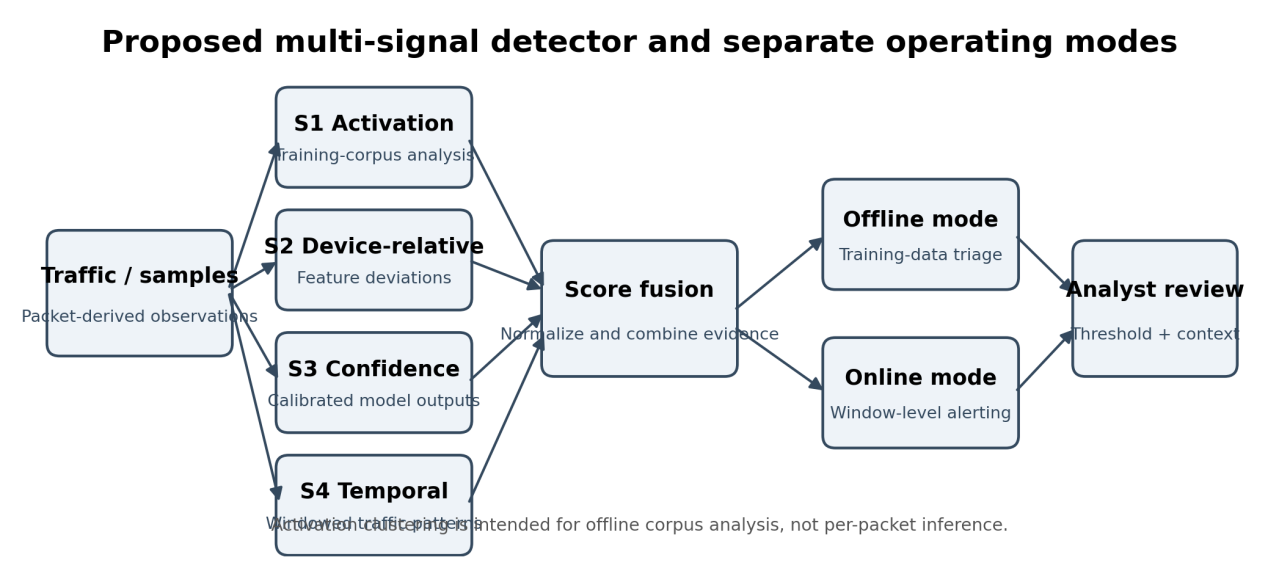
\includegraphics[width=0.92\linewidth]{images/figure2.png}\caption{Proposed multi-signal detection workflow. Offline activation analysis and online traffic monitoring are deliberately separated.}\end{figure}
We propose a detector composed of four evidence channels. The detector is intended to complement, not replace, the original activation-clustering baseline. Two distinct operating modes are defined because training-data sanitization and online traffic monitoring have different information availability and timing requirements.

S1 --- Activation-space analysis Retain the original activation-clustering procedure as the baseline. For a labelled training corpus, extract penultimate-layer representations for samples predicted as benign, apply dimensionality reduction, and cluster the

resulting representations. Cluster assignments and cluster-quality measures are treated as a suspiciousness signal, not as definitive proof of poisoning. The threshold and cluster interpretation must be selected using a validation partition rather than the held-out test set.

S2 --- Device-relative feature consistency For each source device or stable source identity, maintain a baseline distribution for selected packet- and flow-level features, such as packet length, inter-arrival time, packet rate, and jitter. For feature j, a robust standardized deviation can be computed as: zr(j) = [x(j) - median(B\_j)] / [1.4826 x MAD(B\_j) + epsilon] where x(j) is the current observation, B\_j is the reference window for feature j, MAD is the median absolute deviation, and epsilon is a small stabilizing constant. An aggregated feature-consistency score may use a weighted sum or a robust norm of the absolute deviations. The reference window must be constructed using prior or training-only data; it must not include future test observations. Device identity may be unavailable or spoofable, so the design should also report performance when grouping is based on flow or network segment.

S3 --- Prediction-confidence analysis For classifier output probabilities p\_1,...,pC, record maximum softmax confidence and predictive entropy: Cmax = max\_k p\_k       ;   H(p) = -Sigma\_k p\_k log(p\_k) Confidence is only a supporting signal. Backdoored predictions may be highly confident, but so may legitimate predictions; low confidence is not a necessary property of a trigger-bearing sample. Confidence calibration, including temperature scaling where appropriate, should be fitted on validation data and evaluated separately from the detector's discrimination ability.

S4 --- Temporal traffic analysis Within a sliding window, compute indicators such as inter-arrival-time coefficient of variation, short-burst frequency, destination fan-out, packet-size repetition, and short-term prediction changes. These features are motivated by the structured timing and packet-count characteristics of the trigger-generation process. They are not assumed to be unique to malicious traffic: periodic industrial protocols, keep-alive traffic, and legitimate bursts may produce similar patterns. Temporal indicators therefore require per-environment baselines and false-positive analysis.

\paragraph{Fusion and operating modes}
Normalize the S1--S4 outputs using training or validation statistics and combine them with an interpretable lightweight model, initially logistic regression; gradient-boosted trees may be evaluated as a secondary combiner. The fusion model is trained on labelled examples representing clean benign traffic and trigger-bearing traffic, including trigger-bearing examples that the backdoored IDS predicts as benign. To avoid an unrealistic assumption, results should distinguish a supervised oracle setting (where labelled trigger examples are available) from a constrained setting where labels are scarce or unavailable. Performance in the oracle setting must not be presented as evidence that an operational defender can obtain such labels. In training-set sanitization mode, the detector processes candidate training examples and produces a sample-level suspiciousness score before IDS training. In inference-time mode, the system uses only features available at or before the decision time and evaluates traffic in rolling windows. Activation clustering is naturally a batch-oriented training-data analysis; it should not be described as a per-packet real-time detector unless a separate online representation-monitoring mechanism is explicitly defined.

\subsection{Robust adversarial retraining}
\begin{figure}[htbp]\centering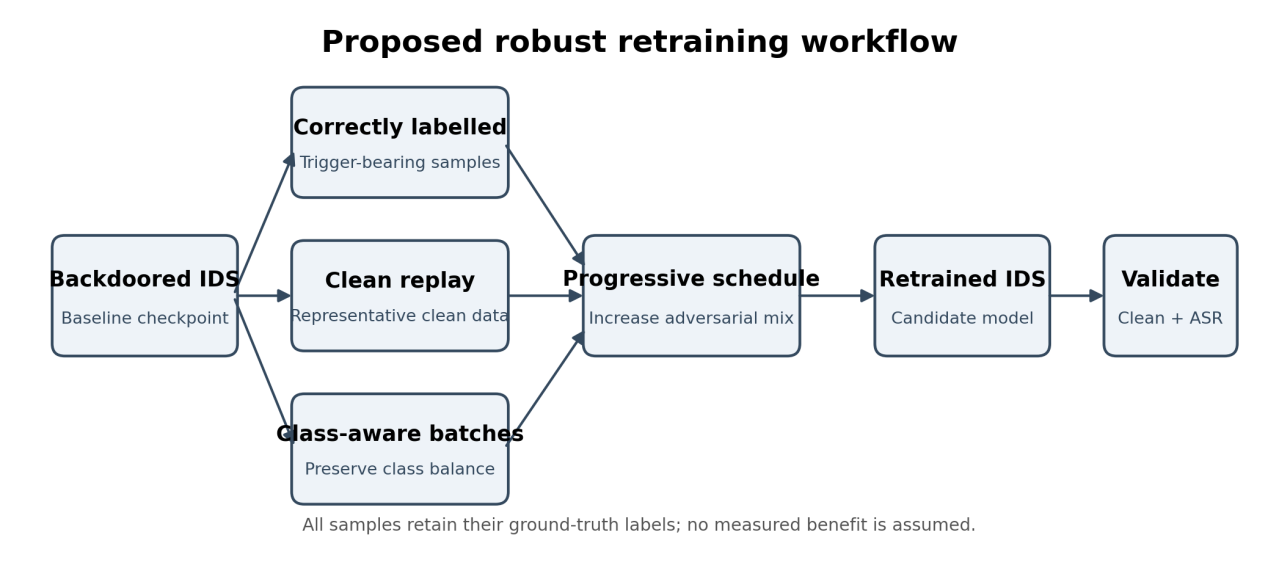
\includegraphics[width=0.92\linewidth]{images/figure3.png}\caption{Proposed robust retraining workflow using correctly labelled trigger-bearing samples, clean replay, class-aware batches, and progressive inclusion.}\end{figure}
We propose a retraining procedure that combines three independently testable components. The objective is to reduce backdoor attack success while preserving clean-task performance, rather than optimizing attack success in isolation.

\paragraph{Class-aware sampling}
Construct mini-batches that preserve representation of each IDS class and separately track clean and trigger-bearing examples. Sampling weights should be selected using the training partition only. Report both class-balanced and naturally distributed evaluation because balancing the training data can change the operational class prior and decision threshold.

\paragraph{Progressive curriculum}
Let q(t) denote the proportion of trigger-bearing defensive examples in epoch t. Instead of introducing the full target proportion at the start, increase q(t) according to a predeclared schedule, for example a linear ramp from zero to qmax over the first K epochs. The values of qmax and K are hyperparameters to be selected on validation data. The curriculum hypothesis is that gradual exposure may reduce abrupt changes to the learned clean decision boundary; this must be tested rather than assumed.

\paragraph{Clean-sample replay}
Maintain a replay buffer of clean training examples, stratified by class where possible. During each retraining epoch, mix replay samples with trigger-bearing defensive examples and the remaining clean training data. The buffer must be sampled only from the training partition, and no test examples may enter retraining. Replay size and mixing ratio should be ablated to quantify the relationship between clean retention, attack success, and training cost.

\paragraph{Combined objective and knowledge settings}
A general training objective can be written as: L(theta) = lambdac Lclean(theta) + lambdaa Ladv(theta) + lambdar Lreplay(theta) where Lclean is the classification loss on ordinary training examples, Ladv is the loss on correctly labelled trigger- bearing defensive examples, and Lreplay is the loss on the clean replay buffer. The coefficients lambdac, lambdaa, and lambdar are selected on validation data. Because the same samples may contribute to more than one term, the implementation must define sampling and weighting precisely to avoid unintended over-counting.

Evaluate two defender-knowledge conditions. In the oracle condition, defensive examples use the same trigger configuration as the attack. In the mismatched condition, defensive trigger parameters differ from those used by the attacker. The latter tests sensitivity to incomplete knowledge of trigger parameters. Both settings should be labelled clearly; neither should be treated as a universal guarantee against unknown triggers.

\subsection{Generalization-aware evaluation}
Three split regimes should be used where the dataset metadata supports them. First, reproduce the original random split for comparability. Second, use a device-disjoint split in which devices or source groups are assigned wholly to one partition. Third, use a chronological split in which earlier traffic is used for training and later traffic is reserved for testing. Where device identity and time are both available, a combined group-and-time split can provide a stricter deployment-oriented test. All preprocessing operations that learn parameters---including imputation, scaling, feature selection, calibration, and detector threshold selection---must be fitted on training data or on a separate validation set. Related packets or flows should be grouped before partitioning where feasible. Any deduplication or grouping rule must be documented because it changes the effective sample distribution. Repeat experiments across multiple independent random seeds, reporting per-seed values, mean, standard deviation, and confidence intervals. Use the same split assignments across compared methods to support paired comparisons. Where additional datasets are considered, require compatibility with the packet-level threat model: a feature-only dataset cannot by itself validate raw-PCAP trigger generation. For Kitsune, the UCI repository documents truncated PCAPNG files; suitability for payload-sensitive processing must therefore be checked and the limitations disclosed \cite{ref10}.

\subsection{Real-time performance evaluation}
Profile the baseline feature-extraction and classifier pipeline, then profile each proposed defense component separately and in combination. Measure per-packet feature-extraction latency, classifier inference latency, detector overhead, and end-to-end decision latency. Report median, 95th-percentile, and 99th-percentile latency rather than only the mean. Measure throughput in packets per second under a stated hardware and traffic-load configuration, CPU utilization during sustained operation, and peak resident memory during training and inference. Define time-to-alert as the elapsed time from the first trigger-bearing observation in a test stream to the first detector alert that satisfies the predeclared alert rule. Report the alert rule, minimum evidence window, and any confirmation count. Measure false alerts per unit time or per number of benign packets in addition to false-positive rate, since operational alert burden depends on traffic volume. Hardware details, software versions, batch/window sizes, concurrency, and warm-up procedures must be disclosed.

\section{Detailed Architecture and Workflow}
The proposed system retains the original PCAP-Backdoor pipeline as its reference path and adds defensive and evaluation modules around it. The architecture is organized into a data plane, model plane, defense plane, and evaluation plane.

RAW PCAP DATA v Packet parsing and traffic grouping v Original feature extraction (e.g., Kitsune-compatible features) v Reference IDS classifier (original DNN) v [--------------------------------------------------------------] | DEFENSE PLANE                                    | | S1 activation analysis | S2 feature consistency         | | S3 confidence analysis | S4 temporal analysis            | |            v                         | |       Lightweight fusion and alert                | |                                      | | Robust retraining: balanced sampling + curriculum + replay | [--------------------------------------------------------------] v Evaluation plane: ASR, clean metrics, detection metrics, generalization splits, latency, throughput, CPU and memory Figure 1. Conceptual architecture of the proposed extension. The figure is a design representation, not an implemented system.

\subsection{Data plane}
The data plane accepts raw PCAP or PCAPNG captures and records capture metadata, source identifiers, timestamps, protocol information, and packet lengths. Traffic is grouped into the units required by the feature extractor and split protocol. Data provenance, capture boundaries, truncation status, and label alignment are retained as metadata. Any packet transformation is applied only in the controlled attack-generation evaluation branch; the clean reference branch remains unchanged.

\subsection{Model plane}
The model plane contains the original feature extractor and reference IDS classifier. The original model is trained under the same split and preprocessing configuration used for the corresponding baseline. Model outputs include predicted class, class probabilities, and the selected hidden-layer representation required by activation-space analysis. Feature normalization parameters and model checkpoints are stored with experiment identifiers to ensure that comparisons use consistent artifacts.

\subsection{Defense plane}
The defense plane has two branches. The pre-training branch analyzes candidate training data and can flag or quarantine suspicious samples before model fitting. The inference branch receives packet-derived features, classifier outputs, and temporal context, then calculates S2--S4 and the fusion score. These branches share feature definitions where possible but have different availability constraints. The robust retraining module is a separate mitigation path: it receives training-only clean and correctly labelled trigger-bearing examples and produces a retrained classifier.

\subsection{Evaluation plane}
The evaluation plane executes the same test cases against the clean baseline, backdoored baseline, original defenses, and proposed extensions. It records classification outcomes, target-class attack success, detection outcomes, split metadata, seed, runtime, and hardware details. All metrics are computed from held-out test data only after model and threshold selection have been completed.

\section{Proposed Evaluation Methodology}
\subsection{Research questions}
\section{RQ1: Does combining activation-space, feature-consistency, confidence, and temporal signals improve backdoor}
detection relative to activation clustering alone?

\section{RQ2: Do class-aware sampling, progressive curriculum inclusion, and clean-sample replay improve the clean-}
performance/attack-success trade-off compared with the original adversarial-retraining procedure?

\section{RQ3: How sensitive are attack and defense conclusions to random, device-disjoint, and chronological data}
splits?

\section{RQ4: What additional latency, throughput reduction, CPU load, and memory use are introduced by the proposed}
detection and retraining components?

\subsection{Experimental conditions and baselines}
Table 4. Planned experimental conditions; these are evaluation plans, not completed results.

Study                                   Conditions                                       Primary outputs S1, S2, S3, S4 individually; selected Detector ablation                                                                        Precision, recall, F1, false-positive rate combinations; full fusion Sampling, curriculum, replay individually Retraining ablation                                                                      Clean accuracy, ASR, per-class recall and combined Random, device-disjoint, chronological Generalization                                                                           Performance gap across partitions splits Oracle and mismatched trigger settings; Robustness                                                                               ASR and detector stability multiple seeds Feature extraction, classifier, detector, full   p50/p95/p99 latency, throughput, CPU, Runtime pipeline                                         memory

The following conditions should be compared using identical data partitions and model configurations: •      Clean reference IDS: trained on unpoisoned training data. •      Backdoored IDS: trained using the original PCAP-Backdoor poisoning procedure. •      Original defense baselines: activation clustering, original adversarial retraining, and neural pruning as described in the source paper, where reproducible configurations are available. •      Proposed detector ablations: S1, S2, S3, and S4 individually; selected pairwise combinations; and full S1--S4 fusion. •      Proposed retraining ablations: class-aware sampling only; curriculum only; clean replay only; each pair; and the combined method. •      Knowledge conditions: oracle trigger parameters and mismatched trigger parameters.

\subsection{Dataset and partition protocol}
\begin{figure}[htbp]\centering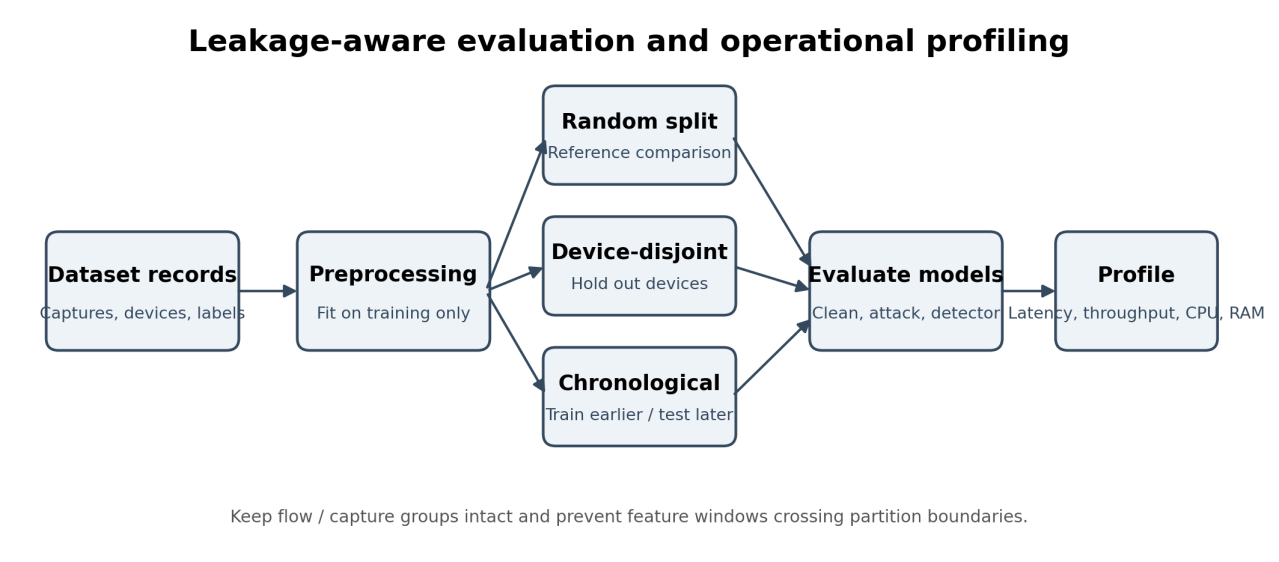
\includegraphics[width=0.92\linewidth]{images/figure4.png}\caption{Proposed leakage-aware evaluation and runtime-profiling workflow.}\end{figure}
Begin with the dataset families used in the original study to preserve comparability. Record the exact capture identifiers, devices, time ranges, attack labels, packet counts, and preprocessing rules. Additional datasets should be selected only if their raw packet representation and labels support the intended packet-level threat model. Feature- only datasets may be useful for classifier generalization studies but cannot independently validate packet insertion or packet-to-feature effects. For each dataset, define train, validation, and test partitions before model development. The random split reproduces the original comparison. The device-disjoint split holds out complete source devices or capture groups. The chronological split trains on earlier traffic and tests on later traffic. Where a dataset has multiple attack captures, keep capture/session groups intact where possible. Report any infeasible split---for example, where too few devices exist---rather than silently substituting a weaker split.

\subsection{Metrics}
Table 5. Metrics to be reported in the proposed evaluation.

Metric                                      Definition / measurement                      Interpretation Correct predictions on unmodified test Clean accuracy                                                                            Preservation of normal IDS utility traffic / all clean test samples Eligible trigger-bearing non-target samples Attack success rate (ASR)                                                                 Backdoor effectiveness predicted as target / all eligible samples Computed for each class and macro- Precision / recall / F1                                                                   Detection/classification balance averaged Benign samples flagged as suspicious / all False-positive rate                                                                       Operational alert burden benign samples p50, p95, and p99 end-to-end processing Latency                                                                                   Per-observation overhead time Throughput                                  Packets or flows processed per second         Processing capacity Deployment cost CPU utilization and peak / steady-state Resource use memory

Evaluation objective                    Metric                                     Interpretation Clean IDS performance                   Accuracy, macro-F1, per-class              Measures ordinary classification quality, precision/recall                           including minority classes. Backdoor effectiveness                  Attack success rate (ASR)                  Fraction of eligible trigger-bearing malicious test samples classified as the attacker-selected target class. Detector quality                        Precision, recall, F1, AUROC, AUPRC,       Measures detection quality; AUPRC is FPR                                        useful when poisoned samples are rare. Defense trade-off                       ASR reduction and clean metric change      Reports security gain together with clean- task cost. Runtime                                 p50/p95/p99 latency, packets/s, time-to-   Measures responsiveness and processing alert                                      capacity. Resource use                            CPU utilization, peak RAM                  Measures deployment overhead on stated hardware.

Table 1. Proposed evaluation metrics. Metric definitions and denominators must be fixed before experiments. For a targeted backdoor, define ASR over eligible trigger-bearing samples whose ground-truth class is not the target class: ASR = number classified as target / number of eligible trigger-bearing samples. Also report the clean accuracy and per-class recall of the same model. Detector precision and recall must use a clearly defined positive class (poisoned or suspicious sample). Report confusion matrices and threshold-specific false-positive rates in addition to threshold-independent curves.

\subsection{Statistical analysis}
Run each experiment across multiple seeds and preserve identical split assignments across competing methods. Report the individual seed results, mean, standard deviation, and 95\% confidence intervals. Use paired comparisons when methods are evaluated on the same test examples. Where statistical tests are used, state the test, assumptions, correction for multiple comparisons, and effect size. Do not infer statistical significance from overlapping or non- overlapping standard-deviation bars alone.

\subsection{Ablation and sensitivity analysis}
For detection, compare each signal independently, the full fusion, and ablations that remove one signal at a time. Vary the detector threshold on validation data and report the resulting precision--recall and false-positive trade-off. For retraining, vary the adversarial-sample proportion, curriculum schedule, replay-buffer size, and loss weights within predeclared ranges. Evaluate both oracle and mismatched trigger settings. For generalization, compare all feasible split types and report performance degradation relative to the random split. For runtime, measure each component in isolation and the complete pipeline under increasing traffic rates.

\subsection{Reproducibility requirements}
An eventual empirical study should disclose dataset versions and provenance, capture identifiers, packet truncation status, label mapping, split manifests, random seeds, preprocessing parameters, model architecture, optimizer settings, stopping rules, thresholds, hardware, software versions, and measurement scripts. All data-dependent transformations must be fitted without using the final test partition. Any excluded captures, failed runs, or deviations from the planned protocol should be recorded.

\section{Discussion}
The proposed extensions address complementary questions rather than one single failure mode. The multi-signal detector tests whether packet-level trigger behavior leaves observable traces outside the classifier's hidden representation. Robust retraining asks whether a defender can reduce the learned association while preserving ordinary IDS behavior. Generalization-aware splits test whether reported attack and defense behavior persists when

traffic sources or time periods are separated. Profiling establishes whether any measured security benefit can be achieved within a realistic resource budget. The detector's main potential advantage is evidence diversity. A trigger may not form a distinct activation cluster yet may produce a measurable temporal or device-relative pattern. However, the signals are not independent: packet rate, jitter, packet size, and classifier confidence may be correlated. A learned combiner can overfit if its training examples do not represent deployment variation. Consequently, the detector must be tested on held-out devices and time periods, and its false-positive burden must be reported. Confidence scores should not be interpreted as calibrated probabilities without calibration testing. The retraining proposal targets a plausible source of clean-performance degradation: changing the training distribution too abruptly or under-representing clean classes. Class-aware sampling, curriculum schedules, and replay may help preserve clean decision boundaries, but they can also reduce the effective diversity of the training data or overemphasize known trigger variants. Oracle retraining is an upper-bound-style condition; mismatched retraining is more informative about incomplete trigger knowledge but still does not cover arbitrary unknown triggers. The split protocol recognizes that different partitions answer different questions. Random splits provide continuity with the original study and measure performance under a shared capture distribution. Device-disjoint splits probe transfer to unseen devices, while chronological splits probe forward-in-time behavior. These settings should be reported separately rather than collapsed into a single score. Not every dataset supports all three partitions, and an unavailable device identity or insufficient temporal metadata must be treated as a limitation. Finally, a real-time detector may require stateful per-source histories and sliding windows. These structures consume memory and may create cold-start behavior for new devices. Profiling should therefore include both steady-state and cold-start conditions, as well as the impact of missing, spoofed, or changing source identifiers. Security effectiveness and operational cost should be considered jointly.

\section{Limitations and Future Work}
This paper is a methodology proposal and has not implemented or evaluated the proposed components. It therefore cannot establish that the multi-signal detector improves detection, that the retraining method reduces ASR without a clean-accuracy penalty, or that the additional evaluation protocol changes the conclusions of the original study. Those are empirical questions reserved for future work. The proposed detector assumes access to training examples or packet-derived observations with sufficient metadata to calculate source-relative and temporal features. In real deployments, source identities may be unavailable, shared, dynamic, or spoofed. Some trigger-related characteristics may overlap with legitimate industrial traffic patterns. Labelled trigger-bearing examples for fusion-model training may also be unavailable to a defender. These constraints require evaluation under both controlled and constrained knowledge settings. The retraining method assumes that correctly labelled trigger-bearing examples can be generated or obtained. This may not hold when the trigger is unknown, when the attacker uses multiple trigger variants, or when generating defensive examples requires knowledge unavailable to the defender. Future work should investigate broader trigger distributions and adaptive attackers, while ensuring that the defense does not merely memorize the specific trigger parameters used in training. Dataset limitations are also important. Public traffic datasets differ in protocol, topology, capture duration, label quality, and packet availability. The Kitsune UCI resource documents PCAP truncation to 200 bytes, which may limit payload-level inspection and must be considered when reproducing packet manipulation \cite{ref10}. Cross-dataset comparison requires careful feature and label harmonization; otherwise, apparent generalization differences may reflect incompatible data collection rather than model robustness. Future work should implement the proposed modules, conduct the full ablation and split-aware evaluation, profile the system on both workstation and resource-constrained gateway hardware, and examine adaptive attackers. Only after these steps should the paper make quantitative claims about detection improvement, robustness, generalization, or deployment feasibility.

\section{Conclusion}
This paper has proposed a structured extension to the PCAP-Backdoor framework focused on detection, robust retraining, generalization, and real-time evaluation. The original packet-level attack and threat model are retained as the reference. The proposed detection methodology combines activation-space analysis with device-relative feature consistency, prediction confidence, and temporal traffic indicators. The proposed retraining strategy combines class- aware sampling, progressive inclusion of correctly labelled trigger-bearing examples, and clean-sample replay. The evaluation protocol adds device-disjoint and chronological splits, repeated runs, leakage controls, and explicit runtime and resource measurements. The central contribution is a testable methodology, not a demonstrated performance improvement. No new experiments or implementation results are reported. The effectiveness and practical value of the proposed extensions remain to be established through controlled, reproducible evaluation. This distinction is essential to ensure that subsequent claims about the security of deep-learning-based network IDS are supported by evidence.

\section*{References}
\bibliographystyle{IEEEtran}
\bibliography{references}
\end{document}
